% !TeX program = xelatex
\documentclass[11pt,a4paper]{article}
\usepackage[margin=22mm,headheight=16pt]{geometry}
\usepackage{fontspec}\setmainfont{TeX Gyre Heros}\setmonofont{TeX Gyre Cursor}
\usepackage{xcolor,graphicx,tikz,tabularx,booktabs,fancyhdr,titlesec,enumitem,listings,hyperref,lastpage}
\usetikzlibrary{positioning,arrows.meta,calc}
\usepackage[most]{tcolorbox}
\definecolor{green}{HTML}{BB652E}\definecolor{soft}{HTML}{FFF8EF}\definecolor{muted}{HTML}{7C838B}\definecolor{blue}{HTML}{EAF1F5}
\definecolor{ink}{HTML}{3C3F46}\definecolor{peach}{HTML}{EB9861}\definecolor{sky}{HTML}{BDD6E8}\definecolor{cream}{HTML}{F9EEDB}\definecolor{line}{HTML}{E8E9E6}
\newcommand{\fitmark}[1][0.15]{\begin{tikzpicture}[x=#1 cm,y=-#1 cm,baseline=-2pt]
\fill[peach](38,10) circle(6);
\fill[peach](9,24).. controls(22,11)and(28,17)..(36,23)..controls(41,27)and(47,25)..(52,22)..controls(48,35)and(35,30)..(29,34)--(9,52)..controls(6,54)and(5,51)..(7,48)--(26,26)..controls(20,23)and(16,22)..(9,24);
\fill[sky](23,43)..controls(39,31)and(49,35)..(48,49)..controls(39,41)and(34,42)..(23,43);
\end{tikzpicture}}
\newcommand{\brand}{\raisebox{5.2mm}[0pt][0pt]{\fitmark[0.012]}\hspace{2mm}{\bfseries\itshape FitCoach AI}}
\newcommand{\chip}[1]{\tikz[baseline=(t.base)]\node[fill=cream,draw=line,rounded corners=2.5mm,inner xsep=3mm,inner ysep=1.5mm,font=\scriptsize,text=green](t){#1};}

\hypersetup{colorlinks=true,linkcolor=green,urlcolor=green,pdftitle={FitCoach AI Product Assembly Guide and User Manual},pdfauthor={Zhang Yancheng}}
\setlength{\parindent}{0pt}\setlength{\parskip}{6pt}
\setlist{itemsep=3pt,topsep=4pt}
\titleformat{\section}{\Large\bfseries\color{ink}}{\tikz[baseline=(n.base)]\node[fill=cream,rounded corners=2mm,text=green,inner sep=7pt](n){\large\thesection};}{0.6em}{}
\titleformat{\subsection}{\large\bfseries\color{green}}{\thesubsection}{0.7em}{}
\pagestyle{fancy}\fancyhf{}\fancyhead[L]{\small\brand\quad{\color{muted}/ Product guide}}\fancyhead[R]{\small\color{muted}LOCAL PROTOTYPE / v1.2}\fancyfoot[L]{\scriptsize\color{muted}YOUR FITNESS COMPANION}\fancyfoot[R]{\small\color{green}\thepage\ {\color{muted}/ \pageref{LastPage}}}\renewcommand{\headrulewidth}{0.3pt}
\newtcolorbox{note}[1]{colback=soft,colframe=line,colbacktitle=soft,coltitle=green,boxrule=0.5pt,arc=3mm,borderline west={2pt}{0pt}{peach},title={#1},fonttitle=\bfseries,breakable}
\lstset{basicstyle=\ttfamily\footnotesize,backgroundcolor=\color{blue},breaklines=true,columns=fullflexible,keepspaces=true,frame=single,rulecolor=\color{soft},showstringspaces=false}
\newcommand{\file}[1]{\nolinkurl{#1}}
\newcommand{\page}[1]{\clearpage\section{#1}}
\tikzset{box/.style={draw=sky,fill=blue,rounded corners=3mm,align=center,minimum height=13mm,text width=36mm,font=\small},flow/.style={-{Latex},thick,draw=green}}
\emergencystretch=3em\relax\sloppy
\begin{document}\color{ink}
\begin{titlepage}
\begin{tikzpicture}[remember picture,overlay]
\fill[cream!35] (current page.north west) rectangle (current page.south east);
\fill[sky!40] ([xshift=-43mm]current page.north east) rectangle (current page.south east);
\fill[peach!20] ([xshift=-15mm,yshift=-28mm]current page.north east) circle(43mm);
\end{tikzpicture}
\brand\hfill\chip{INT4089 / PRODUCT DOCUMENTATION}\par
\vspace{10mm}
{\small\color{muted}YOUR FITNESS COMPANION\par}
\vspace{4mm}
{\fontsize{31}{36}\selectfont\bfseries Product Assembly\\Guide\par}
\vspace{4mm}{\LARGE\color{green}and User Manual\par}
\vspace{5mm}{\color{muted}Sense your movement. Support every repetition.\par}
\vspace{7mm}
\chip{01 / VISION}\hspace{2mm}\chip{02 / MOTION}\hspace{2mm}\chip{03 / FEEDBACK}
\vspace{7mm}
\begin{tcolorbox}[colback=white,colframe=line,arc=4mm,boxrule=0.5pt,left=3mm,right=3mm,top=3mm,bottom=3mm]
{\small\bfseries Your training workspace}\hfill{\scriptsize\color{green}FITCOACH AI}\par\vspace{2mm}
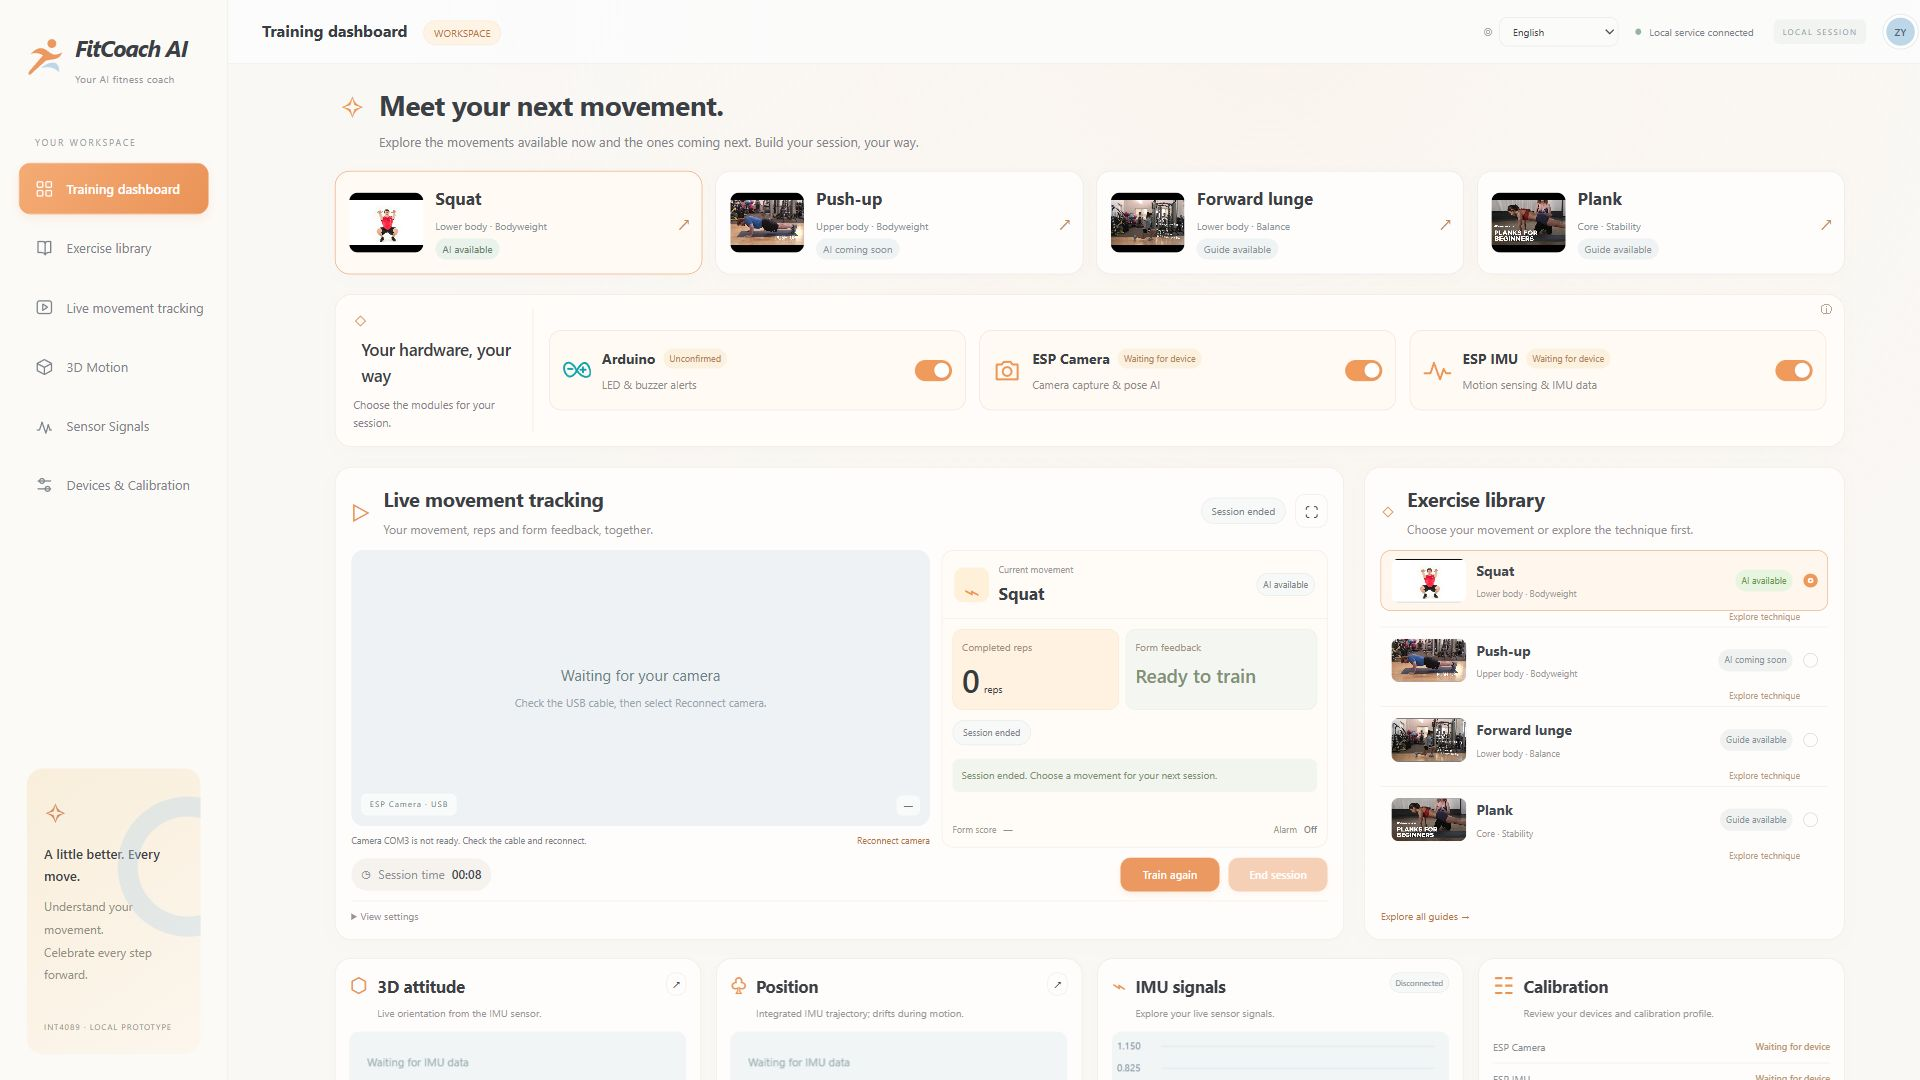
\includegraphics[width=0.88\linewidth]{../assets/fitcoach-ui-en-16x9.png}\par
{\scriptsize\color{muted}Actual interface capture / disconnected-device state}\par
\end{tcolorbox}
\vfill
\vspace{4mm}
{\small Zhang Yancheng\hfill Version 1.2 / 12 November 2026\par}
{\scriptsize\color{muted}Main branch / Assembly, setup and everyday operation\par}
\end{titlepage}
{\footnotesize\setlength{\parskip}{0pt}\tableofcontents}
\page{Product overview and readiness}
FitCoach AI helps demonstrate camera-based squat assessment. An ESP32-CAM sends images to a PC, where YOLOv8n-pose estimates body keypoints and geometric rules evaluate movement. A separate ESP32-S3 relays alarm states to an Arduino. A BMI160 supplies live six-axis motion data through the ESP32-S3 for dashboard visualization.
\begin{note}{What the current product supports}
The unified application enables \textbf{Squat AI}. Push-up and Forward lunge have teaching previews marked AI coming soon. Legacy push-up rules in the source do not make push-up AI available in the current unified launcher.
\end{note}
\par\begin{tabularx}{\linewidth}{@{}l X@{}}\toprule
Subsystem & Readiness at this revision\\\midrule
Vision & Real USB frames and PC inference validated; real exercise accuracy and thresholds still need evaluation.\\
Wireless bridge & ON/OFF, acknowledgements and command expiry validated. An ACK proves S3 receipt only.\\
IMU & Verified on 12 November: address 0x68, chip ID 0xD1; 1,583 samples at 49.74 Hz with zero reported read errors.\\
Physical alarm & Protocol reception has evidence; latest-loop Arduino reception, visible LED and audible buzzer still need on-site acceptance.\\
Cloud & Future direction; no cloud deployment is required.\\\bottomrule
\end{tabularx}
\subsection{Intended use}
Use as a supervised educational prototype in a clear indoor exercise area. Feedback is a rule-based estimate, not a medical assessment or a guarantee of safe form. Stop movement if pain, dizziness or equipment problems occur. Do not rely on the alarm as a protective interlock.
\page{Parts and preparation}
\par\begin{tabularx}{\linewidth}{@{}l c X@{}}\toprule
Part & Qty & Purpose / selection note\\\midrule
ESP32-CAM + OV2640 & 1 & Camera node, supported USB programming/serial connection.\\
ESP32-S3 N16R8 & 1 & 16 MB flash / 8 MB PSRAM target; radio relay and IMU host.\\
BMI160 breakout & 1 & Existing labelled module; verify pin labels before applying the wiring table.\\
Arduino & 1 & Local alarm controller.\\
LED + resistor & 1 each & Series 220 $\Omega$ resistor required.\\
Passive buzzer & 1 & Firmware uses 1600 Hz tone; use a GPIO-compatible low-current device.\\
USB data cables & 3 & One each for CAM, S3 and Arduino. Must support data transfer, not charging only; match each actual socket.\\
Jumper wires / breadboard & As needed & Secure short connections; verify split power rails.\\
PC and camera mount & 1 each & Python environment, USB ports and stable framing.\\\bottomrule
\end{tabularx}
\subsection{Before starting}
\begin{enumerate}
\item Identify every board by its printed label. Record CAM, S3 and Arduino serial ports separately; COM3 and COM4 are examples from the development PC.
\item Inspect cables, loose conductors and exposed pins. Disconnect \textbf{all} USB supplies before adding or moving wires.
\item Keep the repository layout intact: integrated S3 firmware includes the BMI160 source through a relative path.
\item Use the active sketches under \file{firmware/usb-ai-bridge/} and \file{firmware/alarm-mega/}. Historical test sketches replace the active firmware when uploaded.
\end{enumerate}
\begin{note}{Power and logic levels}
Power each controller through its own USB connection. Do not join controller supply pins. Join S3 and Arduino grounds for UART. Never connect Arduino D18 TX to the S3: a reverse 5 V signal needs suitable level conversion. The existing 3.3 V S3-to-Arduino link passed reception tests but is not qualified across worst-case logic tolerances.
\end{note}

\clearpage\subsection{Visual parts reference: controllers and sensor}
These are identification references, not photographs of the assembled prototype. Connector type, PCB layout and pin order may differ by board revision; use the wiring tables and the markings on your own hardware.\par
\newcommand{\partcard}[4]{\begin{minipage}[t]{0.475\linewidth}\begin{tcolorbox}[colback=white,colframe=line,arc=3mm,title={#1},colbacktitle=soft,coltitle=green,fonttitle=\bfseries,boxrule=0.5pt]\centering\includegraphics[width=\linewidth,height=43mm,keepaspectratio]{parts/#2}\par\raggedright\small #3\par\vspace{2mm}{\scriptsize Source: #4}\end{tcolorbox}\end{minipage}}
\partcard{01 / ESP32-CAM + OV2640}{cam.jpg}{Camera node. The camera is shown detached; this board also needs a compatible USB programming/serial interface.}{\href{https://www.flyrobo.in/ai-thinker-s-esp32-cam-bluetooth-wifi-with-ov2640-camera-module}{FlyRobo product photograph}}
\hfill
\partcard{02 / ESP32-S3 N16R8}{s3.jpg}{Motion host and alarm relay. N16R8 identifies memory configuration; it does not uniquely identify a PCB or USB connector.}{\href{https://elektroweb.pl/pl/esp32/1312-modul-esp32-s3-devkitc-1-wroom-1-n16r8-16mb-flash-wifi-bluetooth-usb-c.html}{Elektroweb product photograph}}
\par\vspace{4mm}
\partcard{03 / BMI160 breakout}{bmi160.jpg}{Six-axis IMU. Purple breakout appearance is representative; verify 3v3, VIN, CS and SA0 labels on the actual unit.}{\href{https://www.haljia.com/products/haljia-bmi160-module-6dof-6-axis-rate-angular-velocity-gyroscope-gravity-acceleration-sensor-6-axis-inertial-motion-sensor-purple}{HALJIA product photograph}}
\hfill
\partcard{04 / Arduino}{mega.jpg}{Alarm controller. The reference board has a USB Type-B socket. Compatible boards can use another connector.}{\href{https://store-usa.arduino.cc/products/arduino-mega-2560-rev3}{Arduino official product photograph}}
\par\vspace{3mm}
{\scriptsize\color{muted}Photographs belong to their respective sources and are reproduced here as component identification references. They do not establish electrical compatibility with the prototype.}
\clearpage\subsection{Visual parts reference: cables and small components}
\begin{note}{Three USB data cables are required}
Use one data-capable USB cable for each controller: CAM (through its USB interface), S3 and Arduino. Match the PC end and device end separately. The S3 reference uses USB-C and the Arduino reference uses Type-B; confirm the actual CAM adapter socket. Connector shape alone cannot distinguish a charge-only cable from a data cable. Confirm that each board appears as a serial device.
\end{note}
\begin{center}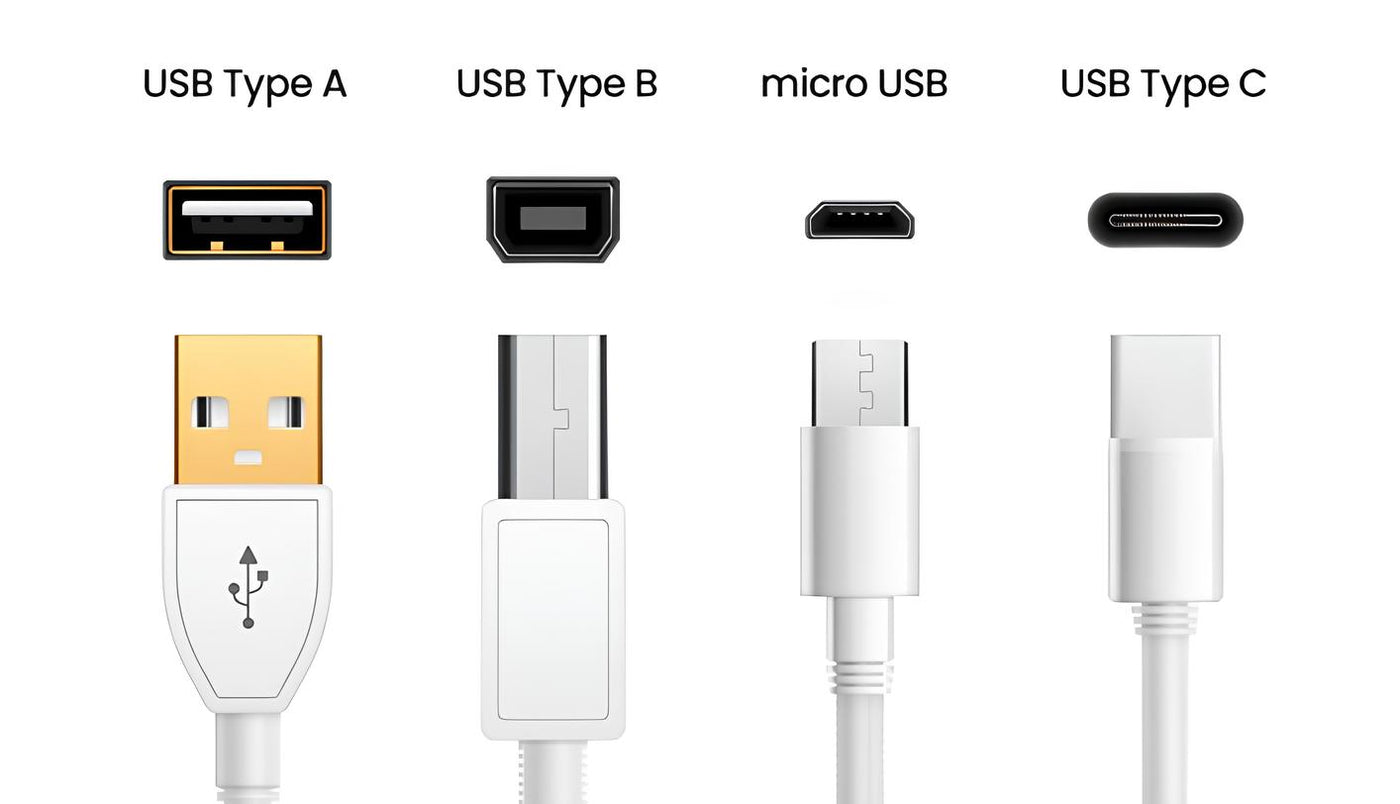
\includegraphics[width=0.85\linewidth,height=44mm,keepaspectratio]{parts/usb.jpg}\end{center}
{\small\textbf{USB connector identification.} Type-A, Type-B, Micro-USB and Type-C appearance examples. Source: \href{https://fr.ugreen.com/blogs/chargeur/principes-de-base-de-lusb-types-vitesse-et-raisons-de-sa-popularite}{UGREEN USB connector guide}.}
\vspace{3mm}
\begin{center}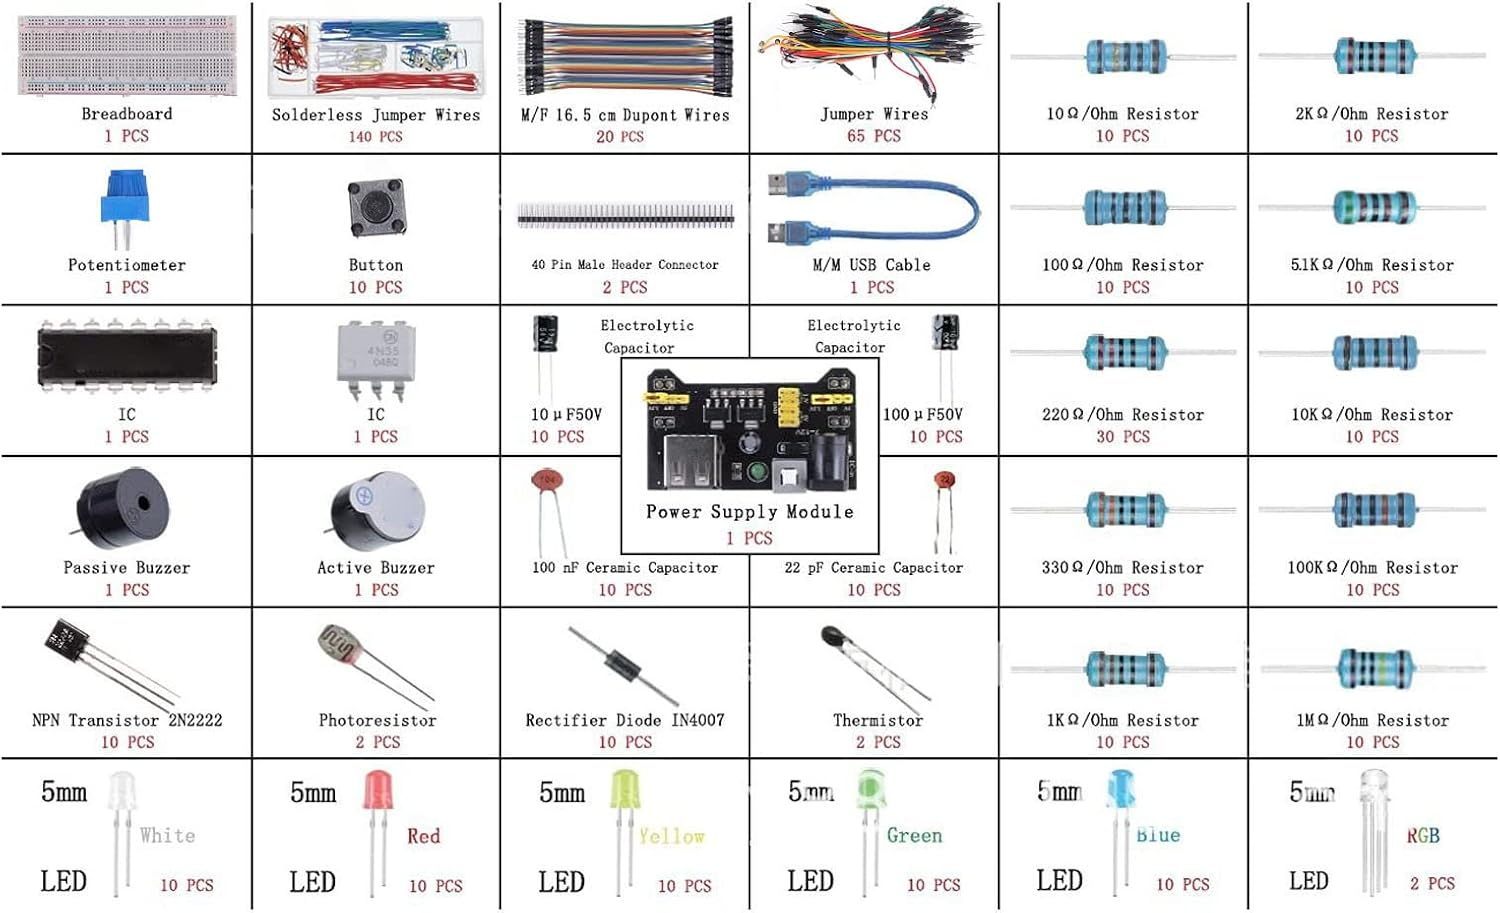
\includegraphics[width=0.95\linewidth,height=65mm,keepaspectratio]{parts/components.jpg}\end{center}
{\small\textbf{Small-component identification.} Reference chart showing breadboard, jumper wires, LEDs, resistors and passive/active buzzers. Use only the parts listed in this manual: one LED, one 220 $\Omega$ resistor, one compatible low-current passive buzzer, breadboard and jumper wires. Other chart items and quantities are not required. Source: \href{https://manuals.plus/asin/B0D929MYW4}{Psytfei kit reference chart}.}
\begin{note}{Check values, not appearance alone}
Measure or read the resistor value; colour and body shape are insufficient. Active and passive buzzers can look alike, so check their type and current rating. Select jumper ends to match the actual headers. The PC and stable camera support are additional equipment, not illustrated electronic components.
\end{note}
\page{System connections at a glance}
\begin{center}
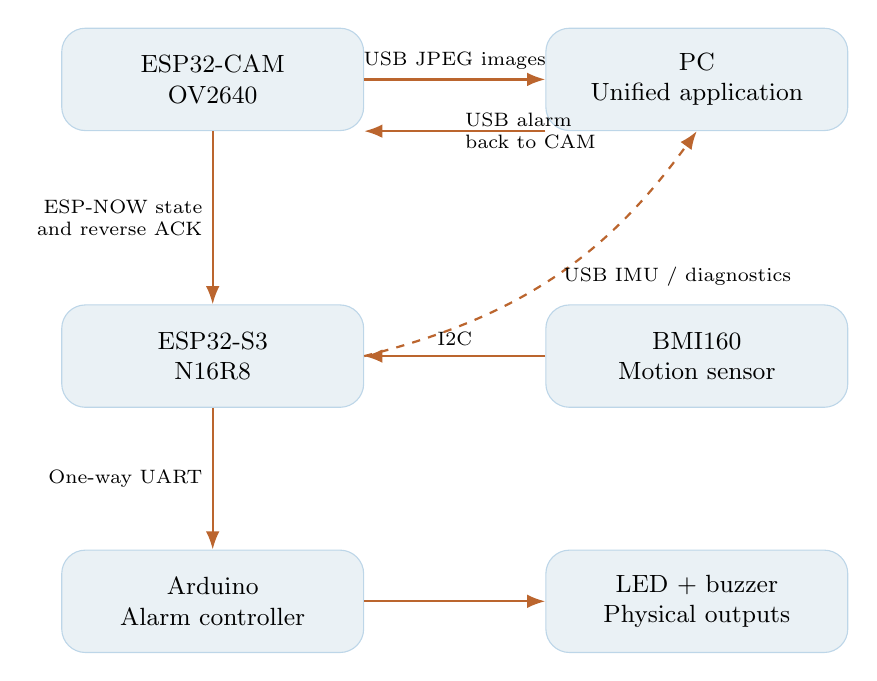
\begin{tikzpicture}[node distance=14mm and 23mm]
\node[box](cam){ESP32-CAM\\OV2640};\node[box,right=of cam](pc){PC\\Unified application};
\node[box,below=22mm of cam](s3){ESP32-S3\\N16R8};\node[box,right=of s3](imu){BMI160\\Motion sensor};
\node[box,below=18mm of s3](Arduino){Arduino\\Alarm controller};\node[box,right=of Arduino](out){LED + buzzer\\Physical outputs};
\draw[flow](cam)--node[above,font=\scriptsize]{USB JPEG images}(pc);
\draw[flow](pc.south west)--node[right,font=\scriptsize,align=left]{USB alarm\\back to CAM}(cam.south east);
\draw[flow](cam)--node[left,font=\scriptsize,align=right]{ESP-NOW state\\and reverse ACK}(s3);
\draw[flow](imu)--node[above,font=\scriptsize]{I2C}(s3);
\draw[flow](s3)--node[left,font=\scriptsize]{One-way UART}(Arduino);
\draw[flow](Arduino)--(out);
\draw[flow,dashed](s3.east) to[bend right=20] node[right,font=\scriptsize]{USB IMU / diagnostics}(pc.south);
\end{tikzpicture}
\end{center}
\textbf{Figure 1.} Functional data paths. Each controller also has independent USB power. Dashed USB telemetry is separate from the alarm radio link; images never travel over ESP-NOW.
\par\begin{tabularx}{\linewidth}{@{}l X@{}}\toprule
Link & Fixed configuration\\\midrule
CAM to PC & 921600 baud, 8N1; 640 $\times$ 480 JPEG, quality 18, two PSRAM buffers, LATEST mode.\\
S3 USB & 115200 baud, 8N1; IMU CSV and diagnostics.\\
CAM to S3 & ESP-NOW channel 1; 20-byte state/ACK packets, 200 ms interval, fixed peers.\\
S3 to Arduino & 9600 baud, 8N1; GPIO17 TX to D19 RX1.\\\bottomrule
\end{tabularx}
\begin{note}{Replacement boards}
Verify the peer MAC addresses in \file{firmware/usb-ai-bridge/AlarmRadio.h} when replacing either ESP32. The CAM target currently expects S3 peer \file{28:84:85:43:72:B0}; S3 expects CAM peer \file{E8:6B:EA:CA:EE:88}. These are current firmware settings, not universal board addresses.
\end{note}
\page{Assembly: motion sensor}
\subsection{Connect the BMI160 with power removed}
This table applies to the existing breakout with separate \file{3v3}, \file{VIN}, \file{CS} and \file{SA0} labels. Another breakout may have a different regulator or pinout. Follow labels rather than wire colour, physical pin count or a mirrored photograph.
\begin{center}
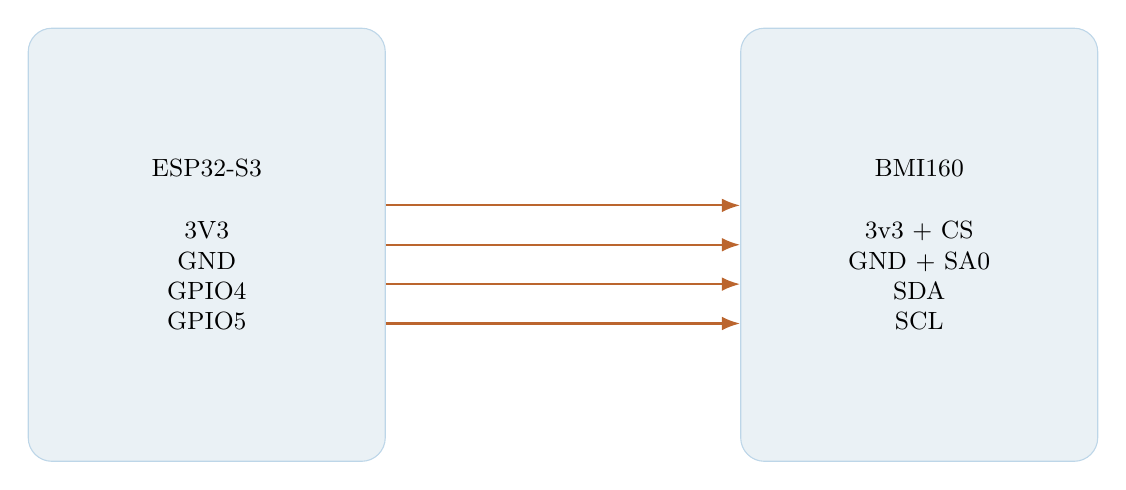
\begin{tikzpicture}
\node[box,text width=43mm,minimum height=55mm](a){ESP32-S3\\[4mm]3V3\\GND\\GPIO4\\GPIO5};
\node[box,text width=43mm,minimum height=55mm,right=45mm of a](b){BMI160\\[4mm]3v3 + CS\\GND + SA0\\SDA\\SCL};
\foreach \y in {5,0,-5,-10}{\draw[flow]([yshift=\y mm]a.east)--([yshift=\y mm]b.west);}
\end{tikzpicture}
\end{center}
\textbf{Figure 2.} Signal-group illustration; the table below is the authoritative connection list. Box text is not a physical pin arrangement.
\par\begin{tabularx}{\linewidth}{@{}l l X@{}}\toprule
S3 & BMI160 & Function\\\midrule
3V3 & 3v3 & Supply the module's 3.3 V rail; leave VIN open.\\
GND & GND & Common reference.\\
GPIO4 & SDA & I2C data.\\
GPIO5 & SCL & I2C clock.\\
3V3 & CS & Hold high for I2C operation.\\
GND & SA0 & Select address 0x68.\\\bottomrule
\end{tabularx}
Leave VIN, OCS, INT1, INT2, SCX and SDX unconnected in this arrangement. CS is not OCS; SDA/SCL are not SDX/SCX. Check breadboard rail continuity before power-up.
\subsection{Mount and verify}
Secure the module without stressing its leads. Record the sensor's axis orientation; body placement and a validated sensor-to-exercise fusion method have not been established. Keep loose bench wiring off the exercising person.

After power-up, the active firmware probes 0x68 and 0x69 and selects the device returning \file{CHIP_ID=0xD1}. With SA0 grounded, the verified unit uses \file{0x68}. On 12 November 2026, the restored integrated firmware produced 1,583 six-axis samples across 31.80 seconds at 49.74 Hz, with zero reported read errors, sequence gaps or non-increasing read timestamps. Wireless reception continued alongside sampling. Keep the ground connection secure and provide strain relief for all sensor leads.
\page{Assembly: alarm and camera}
\subsection{Connect the one-way alarm interface}
\begin{center}
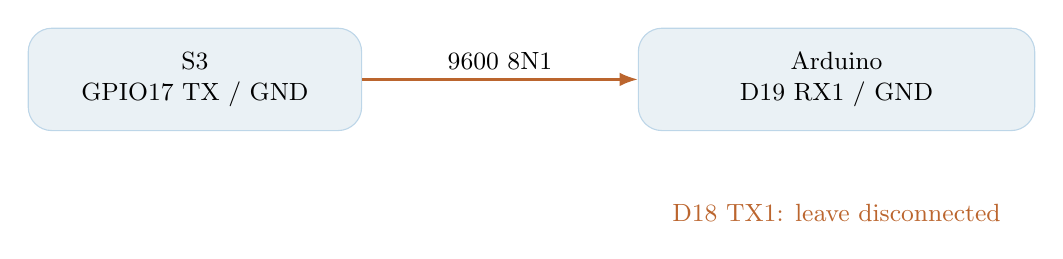
\begin{tikzpicture}[node distance=35mm]
\node[box,text width=40mm](a){S3\\GPIO17 TX / GND};\node[box,right=of a,text width=48mm](b){Arduino\\D19 RX1 / GND};
\draw[flow](a)--node[above,font=\small]{9600 8N1}(b);
\node[below=8mm of b,align=center,font=\small,text=green]{D18 TX1: leave disconnected};
\end{tikzpicture}
\end{center}
\textbf{Figure 3.} UART carries alarm commands only. No return acknowledgement wire exists from Arduino to S3.
\begin{enumerate}
\item With both boards unpowered, connect S3 GPIO17 to Arduino D19 and S3 GND to Arduino GND. Leave Arduino D18 and S3 GPIO18 open.
\item Connect Arduino D8 through a 220 $\Omega$ series resistor to the LED anode; connect LED cathode to Arduino GND. Do not omit the resistor.
\item Connect a compatible low-current passive buzzer positive terminal to D9 and negative terminal to GND. Check its rating first; a higher-current buzzer needs a suitable driver circuit.
\item Inspect for shorts. Connect each board's USB supply independently. Both LED and buzzer should start OFF.
\end{enumerate}
\subsection{Install the camera}
Secure the ESP32-CAM and its USB interface to a stable support. Keep the lens and ribbon connection unobstructed; disconnect power before reseating the camera. The built-in OV2640 wiring is defined by the active CAM sketch, not by the S3 IMU table.

Start at roughly 2--3 m from the user, then adjust so the entire body, including ankles, stays visible throughout the squat. Use even front lighting and an unobstructed exercise area. A side or approximately 45-degree view reveals torso lean better than a pure front view; left/right symmetry is harder to observe from a pure side view.
\begin{note}{Acceptance boundary}
An ESP-NOW ACK confirms S3 receipt, not LED illumination or buzzer sound. Check both outputs directly during commissioning. Startup-OFF and communication expiry are implemented behaviors, not safety-rated protection.
\end{note}
\page{Software installation and firmware}
\subsection{Prepare a new PC}
Install Python and use a dedicated environment. From the repository root:
\begin{lstlisting}
python -m venv app/.venv
app/.venv/Scripts/python.exe -m pip install -r app/requirements.txt
app/.venv/Scripts/python.exe -m serial.tools.list_ports
\end{lstlisting}
The requirements specify dependency ranges, not an exact reproducible lockfile. Prepare the official \file{yolov8n-pose.pt} weights before an offline demonstration. First-time package and weight retrieval needs internet access. A configured development PC can reuse its existing environment.
\subsection{Upload only when needed}
If the active firmware is already installed, do not reflash for normal use. For a fresh build, install Arduino CLI, the Arduino AVR board package and Espressif ESP32 board package. Close the application, serial monitors and test tools first. Confirm board and port identities.
\begin{lstlisting}
arduino-cli compile --fqbn esp32:esp32:esp32cam firmware/usb-ai-bridge/Cam_USB_Bridge
arduino-cli compile --fqbn esp32:esp32:esp32s3:FlashSize=16M,PSRAM=opi,CDCOnBoot=default,USBMode=hwcdc,PartitionScheme=app3M_fat9M_16MB,UploadSpeed=115200 firmware/usb-ai-bridge/S3_IMU_Alarm_Bridge
arduino-cli compile --fqbn arduino:avr:mega firmware/alarm-mega/Mega_Alarm_RX
\end{lstlisting}
Append \file{--upload --port <actual-port>} to the matching command, replacing the placeholder. Uploading replaces the board's existing program. Keep the shared header and included BMI160 source at their original relative locations.
\subsection{Launch the unified application}
From the repository root; substitute your actual CAM and S3 ports:
\begin{lstlisting}
powershell.exe -NoProfile -ExecutionPolicy Bypass -File app/run_pose.ps1 -CamPort COM3 -ImuPort COM4 -Action squat
\end{lstlisting}
Open \url{http://127.0.0.1:8010}. To skip automatic IMU connection, use \file{-ImuPort ''}. The active launcher accepts squat only. Older README examples for pushup or standalone entry points do not describe the current unified experience.
\page{Daily operation}
\subsection{Start a session}
\begin{enumerate}
\item Inspect the assembly and clear the exercise area. Connect the CAM, S3 and Arduino USB cables. Identify ports again after reconnecting.
\item Launch the application and open the local page. Choose English in the header language selector; the browser remembers the preference.
\item Confirm a fresh camera image and check connection indicators. Confirm live IMU updates separately from the radio connection indicator.
\item Stand upright briefly with shoulders, hips and naturally lowered hands visible. Automatic camera direction needs three consistent, sufficiently distinct scans before locking.
\item Select Squat AI from the movement library. Keep the whole body visible and perform a slow trial repetition before a demonstration.
\end{enumerate}
\begin{center}
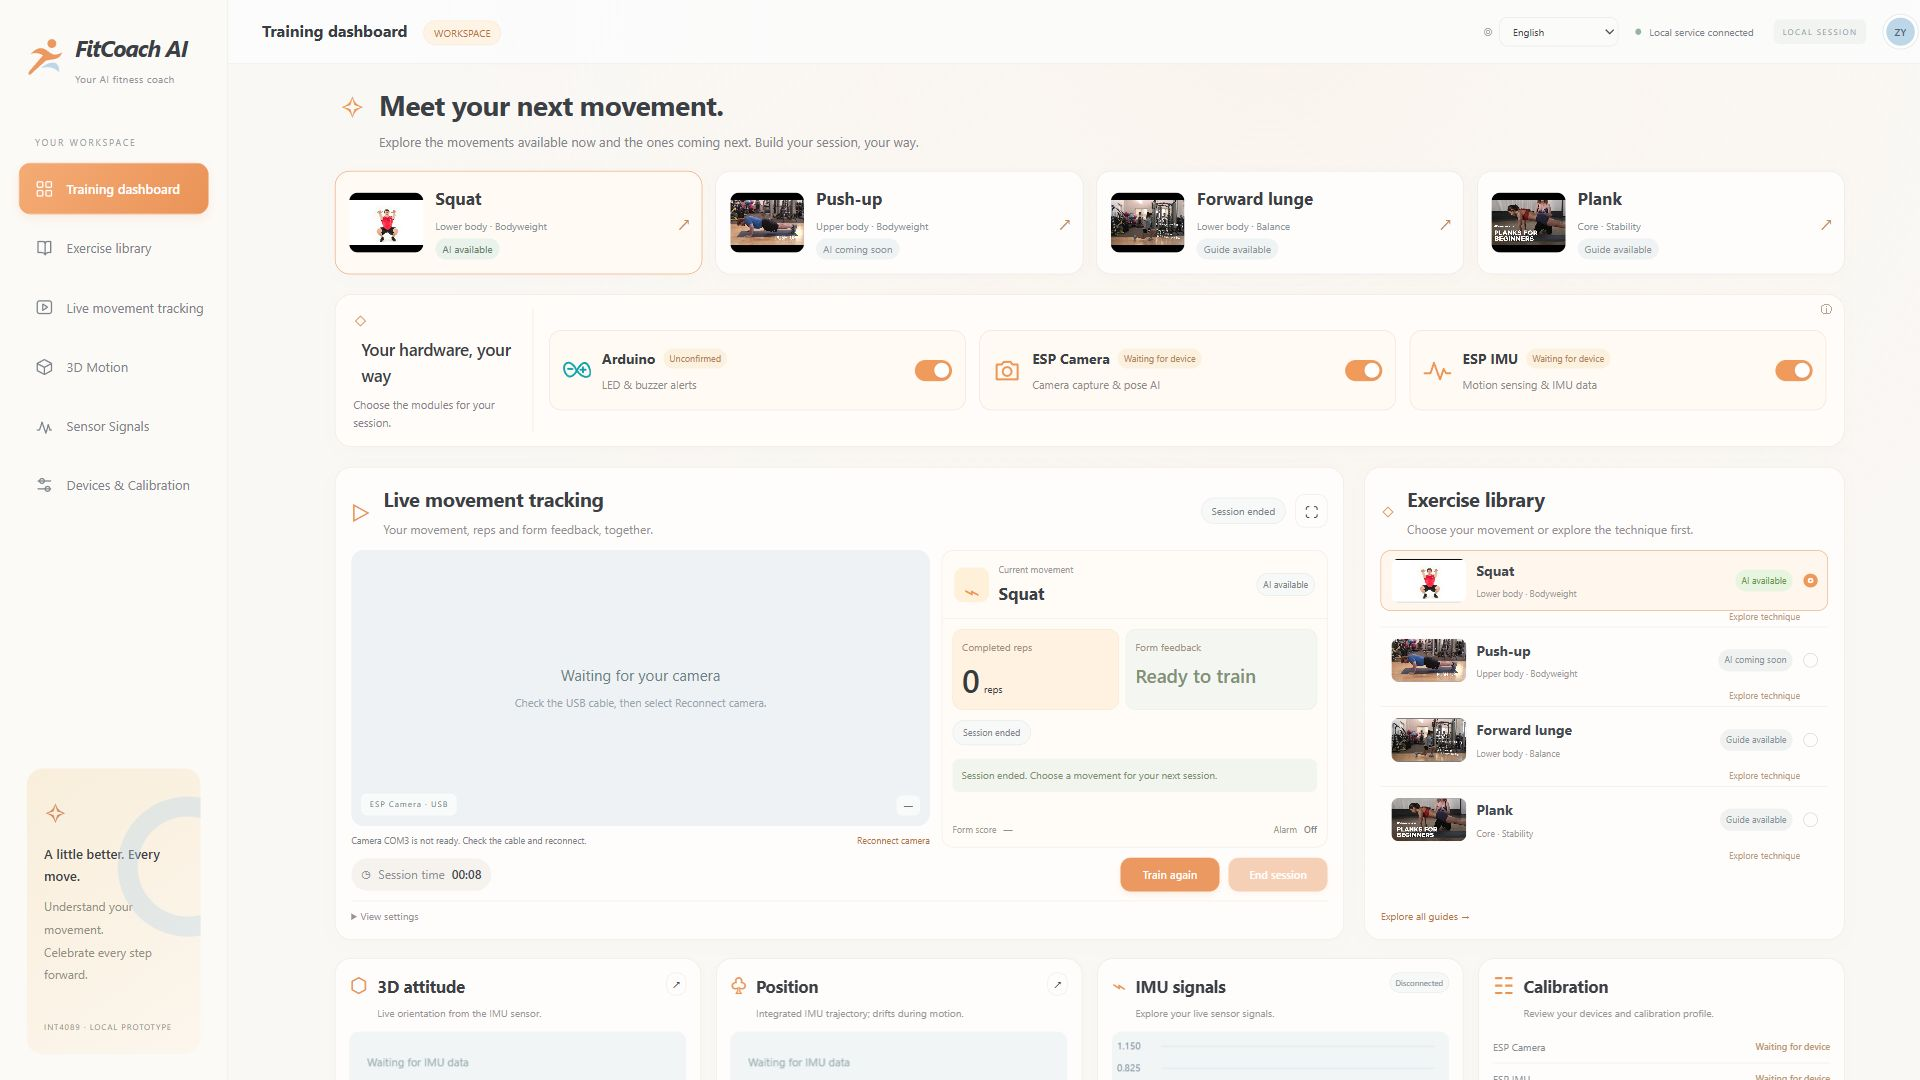
\includegraphics[width=0.88\linewidth]{../assets/fitcoach-ui-en-16x9.png}\par
\end{center}
\textbf{Figure 4.} Repository English dashboard capture. Devices are disconnected in this screenshot; it illustrates the interface, not a successful live session. The four views provide overview, 3D attitude/position, signal charts and connections/replay/calibration.
\subsection{Camera direction and teaching previews}
The default view uses automatic quarter-turn correction and selfie mirroring. After moving the camera, use \textbf{Recalibrate direction}. If automatic orientation is ambiguous, assessment and alarms pause until calibration succeeds; fixed 0/90/180/270-degree overrides are available. Disable mirroring for a conventional or rear-facing view.

Teaching previews explain three movements and may load external videos when clicked. They do not change the AI exercise or alarm state. Push-up and lunge previews are not active AI modes.
\page{Understanding feedback and motion views}
\subsection{Repetitions, scores and alarms}
A repetition is counted on return from descent to standing. The rules track the movement rather than judging a single still frame. A completed repetition with a rule violation produces a two-second alarm event. Missing required keypoints prevents assessment and clears the alarm; no alarm does not prove correct form.
\par\begin{tabularx}{\linewidth}{@{}l l X@{}}\toprule
Squat metric & Current rule & Interpretation\\\midrule
Minimum knee angle & At most 105 degrees & Larger minimum angle is labelled insufficient depth.\\
Maximum torso tilt & At most 45 degrees & Larger tilt is labelled excessive forward lean.\\
Left/right knee difference & At most 20 degrees & Larger difference is labelled asymmetry.\\\bottomrule
\end{tabularx}
These are implementation thresholds in \file{app/form_rules.py}, not validated individual exercise prescriptions. The score is a rule score, not model confidence or an injury-risk percentage. Perspective, occlusion and keypoint jitter affect results; monocular images do not provide a complete 3D biomechanical assessment.
\subsection{Live IMU, replay and calibration}
\begin{enumerate}
\item In Connections, select the S3 port, not the CAM port. Default connection avoids resetting S3; an explicit reset briefly interrupts its radio relay.
\item Check the source label and valid sample status. ``Live'' requires real parsed samples; a connection alone does not prove sensor health.
\item For software demonstrations, load a historical or uploaded CSV and use pause/resume. Replay affects IMU visualization only; live vision continues independently and may still trigger its normal alarm.
\item Import or edit a profile, or calibrate from stationary CSV, only with a trace whose stationary conditions are known. Export JSON to retain changes; session edits do not overwrite repository profiles.
\end{enumerate}
The 3D view displays attitude, gravity, velocity and an integrated position trail. Position drifts during motion because acceleration is integrated twice. Yaw has no magnetometer reference. Position reset changes the origin; it does not improve physical accuracy. Replay displays recorded data and does not generate alarms.
\subsection{End the session}
Stop exercising, stop the server with Ctrl+C, and verify outputs are OFF. On command loss, CAM/S3 leases expire after about 1.2 seconds and Arduino turns outputs off after 1.5 seconds without an accepted frame. These are separate timers, not a guaranteed total shutdown latency. Disconnect all supplies before storage or rewiring.
\page{Commissioning and troubleshooting}
\subsection{Commissioning checklist}
Record date, code revision, board identities, ports and observations. Keep compilation, upload, communication and physical acceptance as separate results.
\par\begin{tabularx}{\linewidth}{@{}l X@{}}\toprule
Check & Pass evidence to record\\\midrule
Power-off inspection & Correct six IMU wires; one-way UART; no joined supply pins; resistor and buzzer rating checked.\\
Camera & Fresh decoded frames with whole-body framing and stable orientation.\\
Vision & Trial repetition counted; feedback matches observed movement. Real accuracy still needs a labelled evaluation.\\
Radio & ON/OFF and S3 ACK observed; document command-expiry behavior.\\
Actuators & Arduino receives commands; LED visibly changes and buzzer audibly changes in the latest loop.\\
IMU & Verified identity 0xD1 at 0x68; continuous six-axis samples at approximately 50 Hz.\\
Loss cases & Observe actual USB/radio/power-loss behavior; do not infer it solely from software tests.\\\bottomrule
\end{tabularx}
\subsection{Common problems}
\par\begin{tabularx}{\linewidth}{@{}p{35mm} X@{}}\toprule
Symptom & Action\\\midrule
Port busy / upload fails & Stop the app, serial monitor and standalone tools. Only one process can own a port.\\
No camera image & Check USB data cable and actual CAM port. Use camera reconnection in the page; re-identify the port after reconnecting.\\
No repetitions & Check full-body framing, lighting, Squat selection and orientation lock. Ankles outside the image prevent knee-angle assessment.\\
S3 ACK absent & Check both nodes are powered, correct active firmware, fixed peer MACs and channel 1. Images may still work over USB.\\
ACK present, no alarm & Check S3 GPIO17 to Arduino D19 and common ground. Check Arduino firmware, LED polarity, resistor and buzzer rating. ACK is not actuator feedback.\\
IMU port selection & Select the S3 port (COM4 on the verified PC), 115200 baud, and live input. Close other serial tools before connecting.\\
Position drifts & Expected integration limitation; reset origin for viewing. Do not interpret the trail as measured absolute position.\\\bottomrule
\end{tabularx}
\page{Maintenance and technical reference}
\subsection{Care and records}
Store the assembly dry and unpowered; protect the lens and avoid pulling sensor leads. Before each demonstration, inspect connections and repeat the basic camera/actuator checks. Keep credentials and identifiable camera recordings out of version control. The unified integration does not save raw camera frames by default.
\subsection{Alarm interface for maintainers}
Arduino accepts exactly three ASCII binary digits plus LF (CRLF accepted): source, state, source-XOR-state. PC USB is source 0 at 115200 baud; S3 UART is source 1 at 9600 baud.
\begin{center}\begin{tabular}{lll}\toprule
Frame + LF & Input & Meaning\\\midrule
\file{000} & PC USB & OFF\\
\file{011} & PC USB & ON\\
\file{101} & S3 UART & OFF\\
\file{110} & S3 UART & ON\\\bottomrule\end{tabular}\end{center}
For a supervised direct Arduino test, stop competing tools, open its actual port in Serial Monitor at 115200 with newline ending, wait about two seconds after opening, then send \file{011} and \file{000}. A single accepted command lasts only 1.5 seconds; a 200 ms heartbeat sustains control. Direct PC commands take priority over S3 for 1.5 seconds. An OFF command is not a physical disconnection of power.
\subsection{Evidence and source map}
This edition follows the main-branch application and the integrated S3/IMU verification performed on 12 November 2026. Relevant repository files:
\begin{itemize}
\item \file{README.md}; \file{app/UNIFIED_APP.md}; \file{app/run_pose.ps1}: current architecture, interface and launch behavior.
\item \file{firmware/usb-ai-bridge/}: active CAM/S3 sketches and \file{AlarmRadio.h}; \file{firmware/alarm-mega/Mega_Alarm_RX/}: actuator code.
\item \file{firmware/esp32-camera/BMI160_WIRING.md}: six-wire breakout connection reference.
\item \file{docs/protocols/}: USB, ESP-NOW and alarm contracts.
\item \file{docs/validation/2026-11-10-camera-speed-after.json}: USB-only 268 frames in 30 seconds, 8.93 FPS, no CRC/decode errors. This is not guaranteed AI throughput.
\item \file{docs/validation/2026-11-11-unified-app.json}: unified application validation scope. Interface and software checks; live IMU verification is recorded separately below.
\item \file{docs/validation/2026-11-12-imu-restored.json}: integrated IMU acquisition and passive wireless reception results.
\end{itemize}
\end{document}
